% Class:
\documentclass{beamer}
\usetheme{Darmstadt}
\usecolortheme{seahorse}

% Fonts:
\usepackage[T1]{fontenc}
\usepackage{lmodern}
\usefonttheme{serif}

% Links:
\usepackage{hyperref}

% Maths:
\usepackage{amsmath}
\usepackage{amssymb}
\usepackage{mathrsfs,amsmath}
\newcommand{\e}[1]{\times 10^{#1}}
\usepackage{siunitx}

% Algorithms:
\usepackage{algorithm}
\usepackage{algpseudocode}

% Figures:
\usepackage{graphicx}
\usepackage{caption}
\usepackage{subcaption}
\graphicspath{ {./} }
\usepackage{float}

% Footnotes:
\usepackage[symbol]{footmisc}
\renewcommand{\thefootnote}{\fnsymbol{footnote}}

% Others:
\usepackage{pdfpages}
%\usepackage[backend=bibtex]{biblatex}
\usepackage{textcomp}
\usepackage{pdflscape}
%\usepackage{titling}

% Title:
\title{
	Sound-source Localisation using a Microphone-array for NUbots\\
	Interim Report
}
\author{Clayton Carlon, C3327986}
\date{\today}

\begin{document}

\frame{\titlepage}

\section{Introduction}

% Locating a source of sound is a long sought after ability in technology, especially in the study and development of robotics which seeks to emulate and compete with human senses. The main aspiration for this project is to develop an array of microphones along with an accompanying computation, preferably embedded, to locate a source of sound using signal-processing techniques. In the end, this system will be used on the football-playing robots in the NUbots team, the university's on-campus robotics team. Therefore, the problem for this project to solve is to develop a sound-source-localisation technique using a combination of electronics, embedded computing, and signal-processing so that the robots can locate events on the field and possibly interact with and selectively listen to humans.

\begin{frame}
\frametitle{Problem and Background}

To locate a sound-source akin to that of humans is a long sought after ability in technology.\\

The problem is:
\textit{to develop a sound-source-localisation technique on an array of microphones using a combination of electronics, embedded computing, and signal-processing.}\\
	
\begin{columns}

\column{0.7\textwidth}
Ideally, the system will be used on the robots in the NUbots team to locate acoustic events on the field and possibly interact with humans.

\column{0.3\textwidth}
\begin{figure}[H]
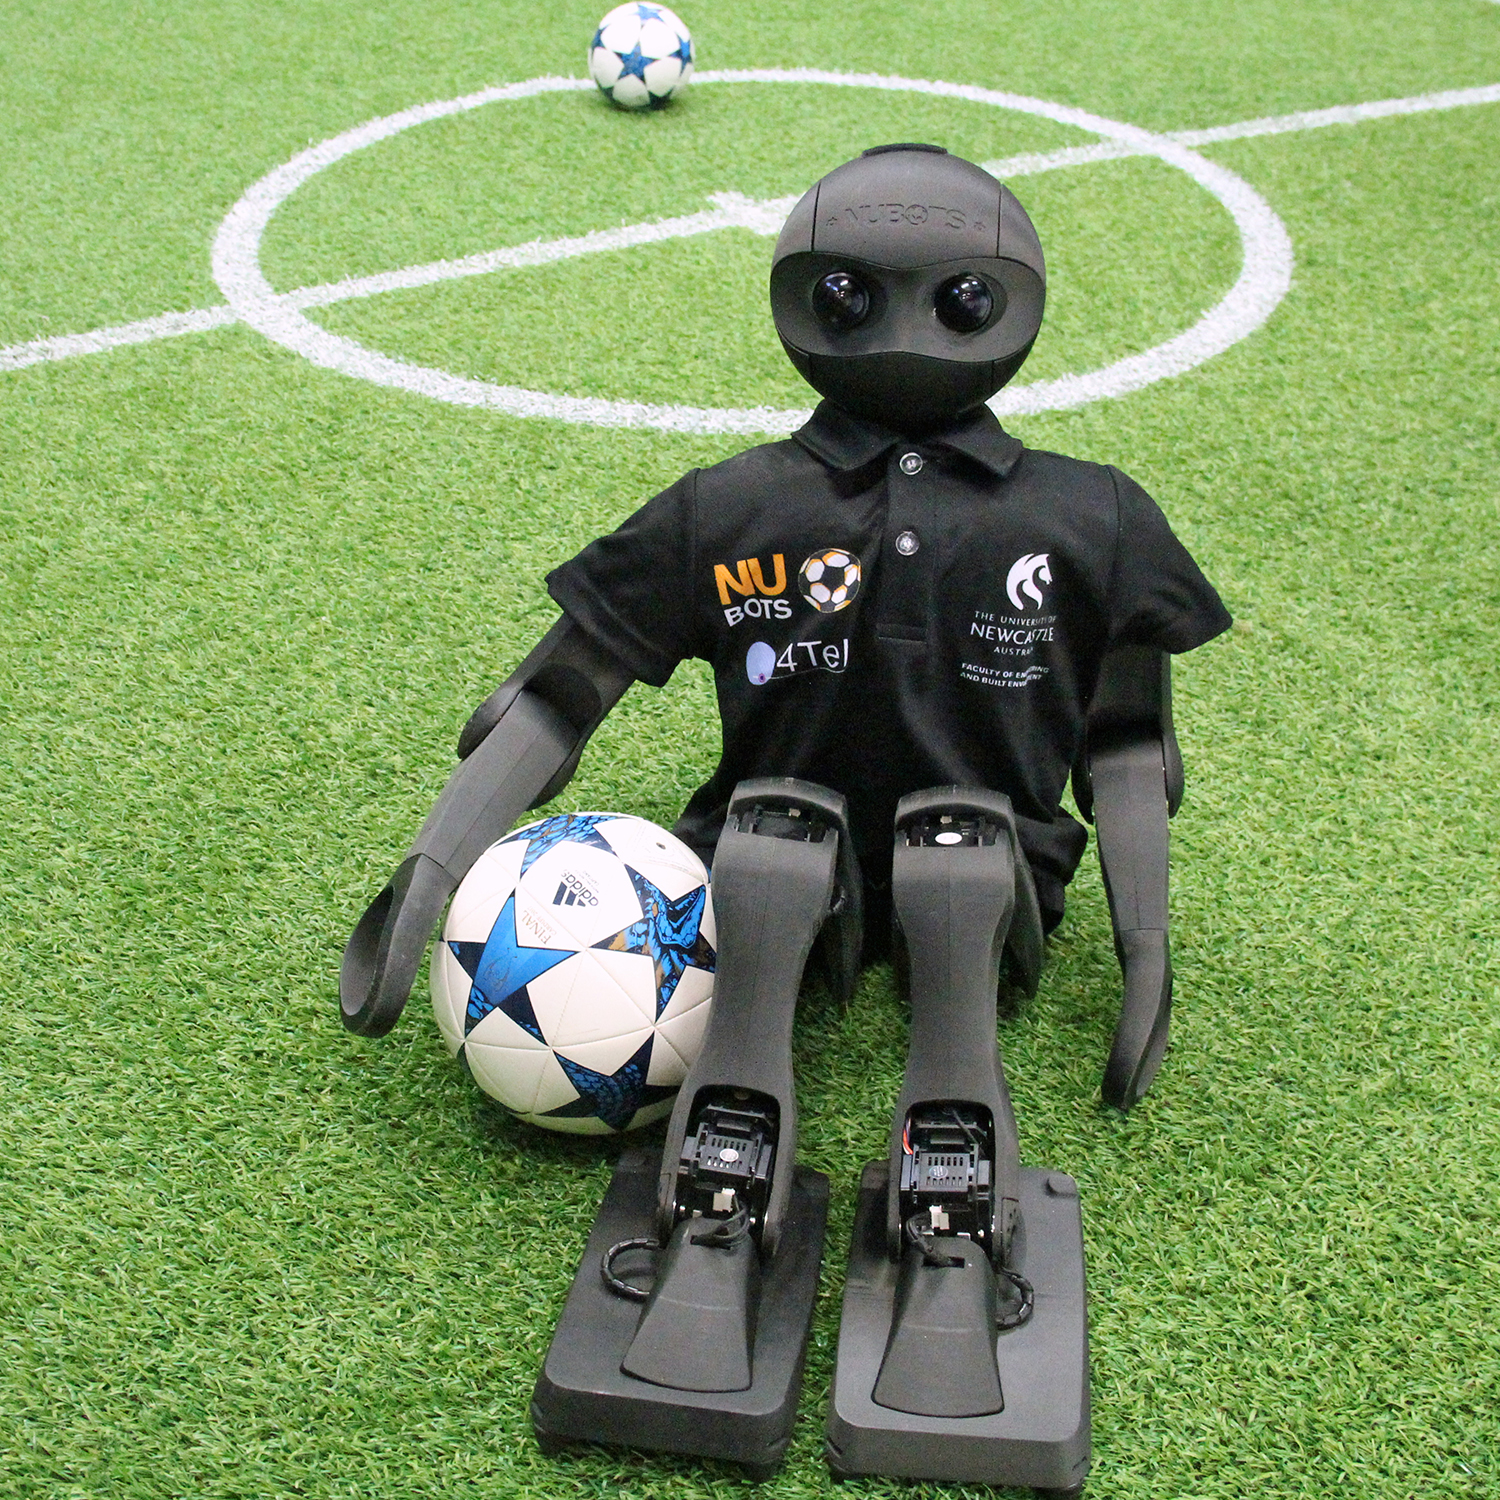
\includegraphics[width=0.9\textwidth]{./NUbot-sitting-down.jpg}
\centering
\end{figure}

\end{columns}

\end{frame}

\begin{frame}
\frametitle{Scope}

Essentially, the system should:
\begin{itemize}
	\item estimate the three-dimensional direction,
	\item locate a reasonably distinct sound in a moderate environment, e.g. a whistle, a lone voice, a loud thud,
	\item and handle the noise from the motors.
\end{itemize}
Ideally, it can:
\begin{itemize}
	\item estimate the distance along with direction,
	\item track the location over time using e.g. a Kalman filter,
	\item locate multiple simultaneous sources,
	\item spatially filter the localised sound,
	\item and work well enough in noisy and reverberant environments, e.g. in a hall full of people.
\end{itemize}

\end{frame}

\section{Literature-Review}

\begin{frame}
\frametitle{Main Methods}
Only classical signal-processing methods are reviewed.

Three main methods in the literature are:
\begin{itemize}
	\item time-difference of arrival (TDOA),
	\item beamforming,
	\item and multiple-signal-classification (MUSIC).
\end{itemize}

\end{frame}

\subsection{Time-Difference Of Arrival}

\begin{frame}
\frametitle{Time-Difference of Arrival}

A simple yet proven way to estimate the direction or the location is to measure the time-delay or TDOA between microphones. For example, a basic formula is:
\begin{equation}
\theta = \sin\left( \frac{c\Delta t_{ij}}{d_{ij}} \right)
\end{equation}
\tiny{where $c$ is the speed of sound, and $d_{ij}$ is the displacement between the microphones, and assuming that the source is in the far field.}

\begin{figure}[H]
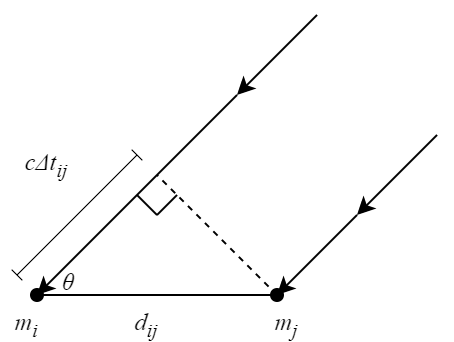
\includegraphics[width=0.4\textwidth]{./basic_tdoa.png}
\centering
\end{figure}

\end{frame}

\begin{frame}
\frametitle{Cross-Correlation}

The most common way to compute the TDOA is to find the peak of the cross-correlation of two signals $x_i$ and $x_j$:
\begin{equation}
R_{ij}(\tau) = \sum_{n=0}^{N-1} x_i[n]x_j[n-\tau] = \mathfrak{F}^{-1} \left( X_i[k]X_j[k]^* \right)
\end{equation}
\tiny{where $X_i$ and $X_j$ are the Fourier transforms of two signals.}\\\small

The generalised cross-correlation (GCC) is:
\begin{equation}
R^{(w)}_{ij}(\tau) = \mathfrak{F}^{-1} \left( \psi[k]X_i[k]X_j[k]^* \right)
\end{equation}
\tiny{where $\psi[k]$ is a spectral weighting.}\\\small

A common weighting is to whiten the whole spectrum which is known as the phase-transform (PHAT) \cite{argentieri_survey_2015}, \cite{rascon_localization_2017}. This is known to improve accuracy especially against reverberation.
\end{frame}

\begin{frame}
\frametitle{Generalised Cross-Correlation and Phase Transform}

\begin{figure}[H]
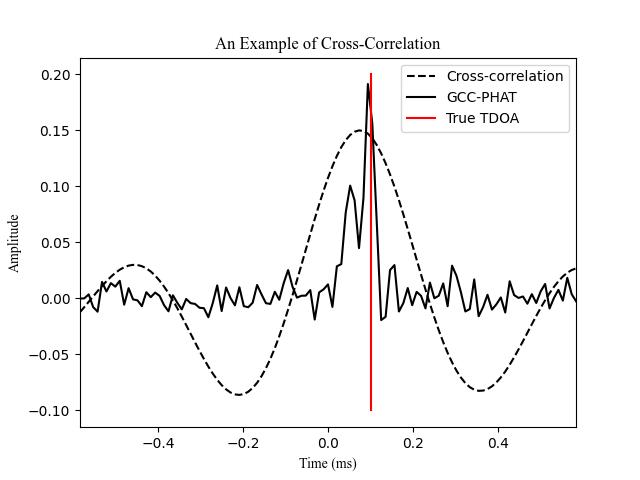
\includegraphics[width=0.6\textwidth]{../Python/gcc_phat/gcc_example.png}
\centering
\end{figure}

\begin{itemize}
	\item The resolution can be improved with up-sampling.
	\item There is a peak at zero for narrowband signals and high noise.
\end{itemize}

\end{frame}

\begin{frame}
\frametitle{Literature-example}

Chen \& Xu (2019), \textit{A Sound Source Localization Device Based on Rectangular Pyramid Structure for Mobile Robot} \cite{chen_sound_2019}

\begin{columns}

\column{0.7\textwidth}
\begin{itemize}
	\item Estimated distances up to 6 \si{m} as well as direction.
	\item Used a slightly modified PHAT to deal with reverberation.
	\item At worst, the error in distance was 0.4 \si{m} for an SNR of 10 \si{dB}.
	\item The error in azimuth was within 1.5 \si{\deg}.
\end{itemize}

\column{0.3\textwidth}
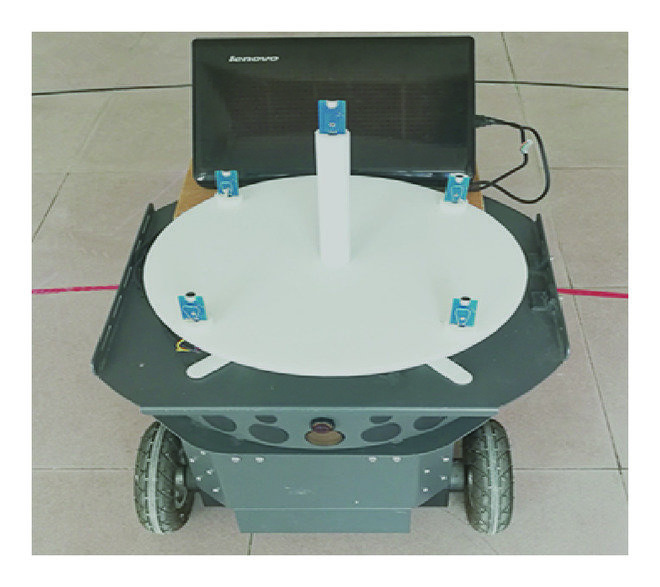
\includegraphics[width=0.9\textwidth]{./chen_2019/array.jpg}\\
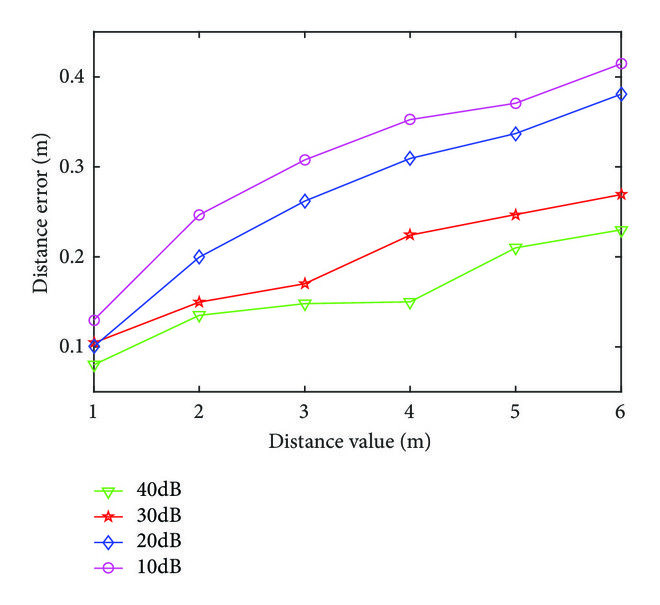
\includegraphics[width=1.0\textwidth]{./chen_2019/distance_SNR.jpg}
\cite{chen_sound_2019}

\end{columns}

\end{frame}

\subsection{Beamforming}

\begin{frame}
\frametitle{Beamforming}

Is a very common signal-processing technique. Signals from many microphones are delayed such that they constructively interfere given a direction or location and form a beam.

The basic beamformer is the delay-and-sum kind \cite{argentieri_survey_2015}.
\begin{equation}
y_{\vec{u}_0}[t] = \sum_{m=1}^M x_m[t-\tau_m(\vec{u}_0)] 
\end{equation}
\tiny{where $\tau(\vec{u}_0)$ is the time-delay at the $m$-th microphone corresponding at the direction $\vec{u}_0$.}\\\small

\begin{columns}

\column{0.6\textwidth}
Given a grid of directions, this output can yield an energy-map as:
\begin{equation}
E_{\vec{u}_0} = \sum_{t=1}^T y_{\vec{u}_0}[t]^2
\end{equation}

\column{0.4\textwidth}
\begin{figure}[H]
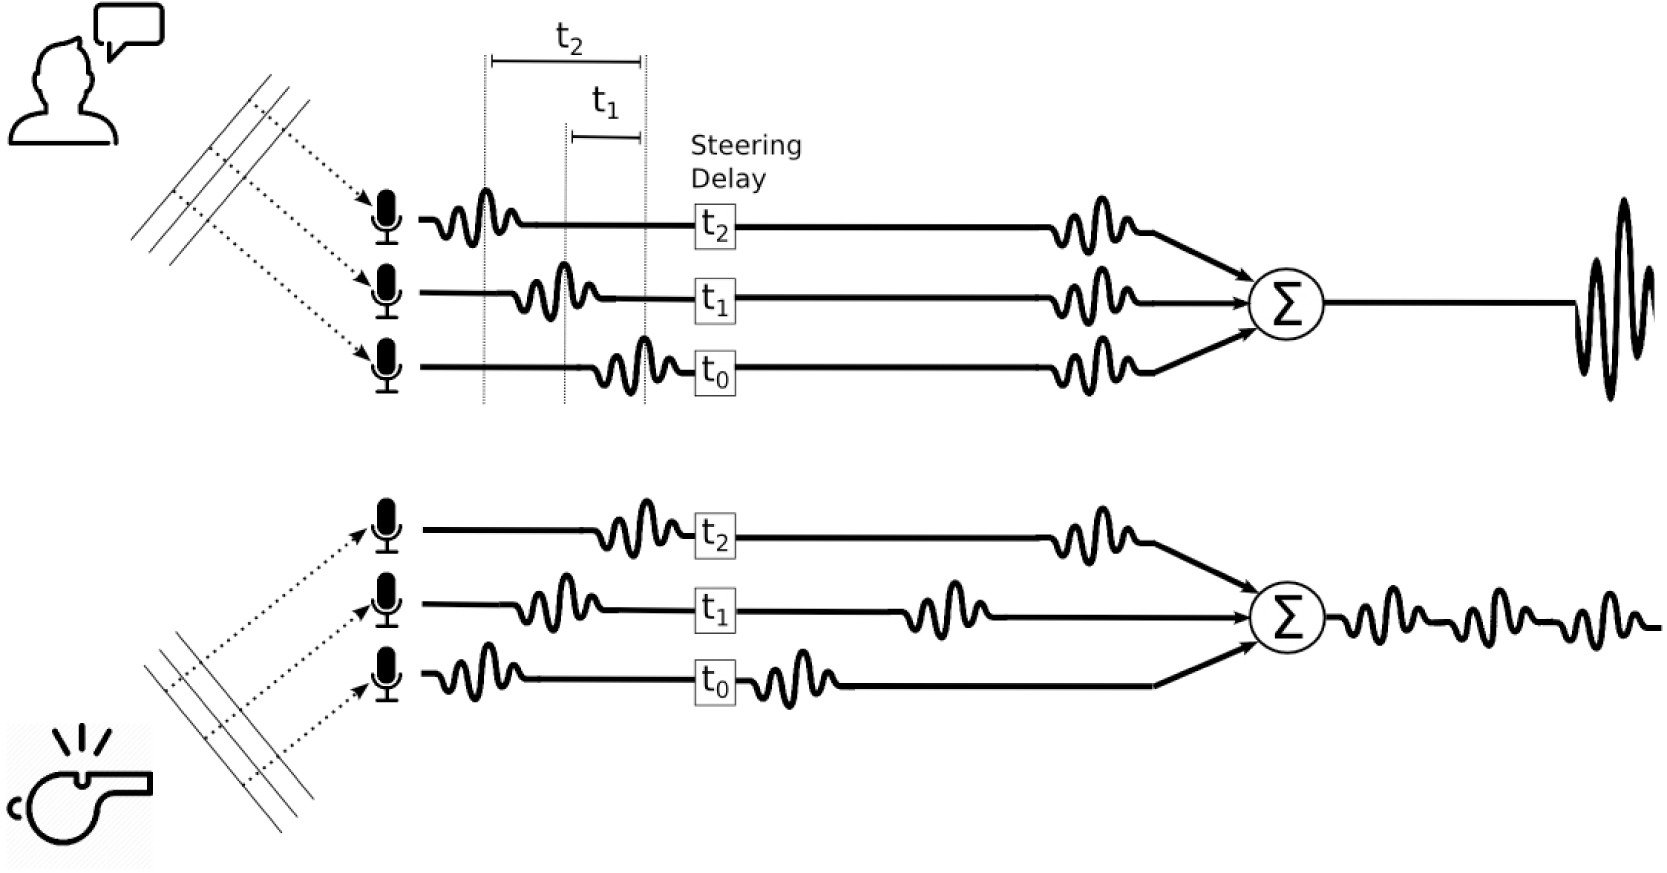
\includegraphics[width=0.9\textwidth]{./rascon_2017/delay_and_sum.jpg}
\centering
\end{figure}
\cite{rascon_localization_2017}

\end{columns}

\end{frame}

%\begin{frame}
%\frametitle{Steered Response Power}
%
%The same delay-and-sum beamformer can be mathematically rewritten as a sum of cross-correlations:
%\begin{equation}
%E_{\vec{u}} = K 
%+ 2 \sum_{m_1=1}^M \sum_{m_2=1}^{m_1-1} R_{m_1,m_2} (\tau_{m_1}(\vec{u}_0) - \tau_{m_2}(\vec{u}_0))
%\end{equation}
%where $K$ is nearly always constant. Many of the same techniques used in TDOA-based methods are used here, e.g. spectral weighting (SRP-PHAT), FFT, etc.
%
%\end{frame}

\begin{frame}
\frametitle{Literature-example}

Valin et al. (2007), \textit{Robust Localization and Tracking of Simultaneous Moving Sound Sources Using Beamforming and Particle Filtering} \cite{valin_robust_2007}

\begin{columns}

\column{0.6\textwidth}
\begin{itemize}
	\item Whitened the spectrum.
	\item Used a spherical search-grid of 2562 points which gave a resolution of 2.5 \si{\deg}.
	\item Applied a particle filter.
	\item Switched between a coarse and a fine search grid to improve the resolution.
	\item At worst, the errors in azimuth and elevation were 1.10 and 1.44 \si{\deg}.
\end{itemize}

\column{0.4\textwidth}
\begin{figure}[H]
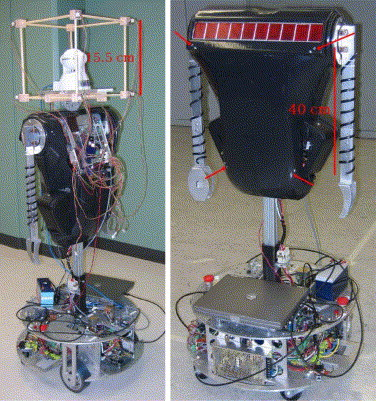
\includegraphics[width=0.9\textwidth]{./valin_2007/array.jpg}
\centering
\end{figure}
\cite{valin_robust_2007}

\end{columns}

\end{frame}

\subsection{Multiple-Signal Classification}

\begin{frame}
\frametitle{Multiple-Signal Classification}

Separates the space of signals into two subspaces, namely one for signals and another for noise. This is done through the eigen-decomposition of the sampled covariance matrix $R[f]\in \mathbb{C}^{N\times N}$. There are broadly three kinds, namely:
\begin{itemize}
	\item standard eigen-value decomposition (SEVD),
	\item generalised eigen-value decomposition (GEVD),
	\item and generalised singular-value decomposition (GSVD).
\end{itemize}

Tends to have very high-resolution and robustness to noise and interference but is very computationally heavy.

\end{frame}

\begin{frame}
\frametitle{Generalised Eigen-Value Decomposition}

In GEVD, the eigen-decomposition is done on:
\begin{equation}
K^{-1}[f] R[f] = Q[f] \Lambda[f] Q^{-1}[f]
\end{equation}
\tiny{where $\Lambda[f]$ is a diagonal matrix of the $M$ eigenvalues $\lambda_m[f]$, and each column of $Q[f]$ is a corresponding eigenvector $q_m[f]$ \cite{nakamura_real-time_2012}.}\\\small

This matrix of eigenvectors is often split into two subspaces, $Q[f] = [Q_s[f]|Q_n[f]]$. Also, $K[f]$ is a freely chosen matrix but is often computed as $N[f]N^*[f]$ where $N[f]$ is the frequency-domain noise recorded when there are no signals.

Like beamforming, an energy-map is drawn:
\begin{equation}
P(\theta_0, \phi_0)[f] = \frac{\lvert A^*(\theta_0, \phi_0) A(\theta_0, \phi_0) \rvert}
	{\sum_{m=\tilde{N}+1}^M \lvert A^*(\theta_0, \phi_0) q_m[f] \rvert}
\end{equation}
\tiny{where $\tilde{N}$ is the number of sources considered, and $A(\theta_0, \phi_0)\in \mathbb{C}^{M\times 1}$ is the steering vector.}\\\small

\end{frame}

\begin{frame}
\frametitle{Literature-example}

Nakamura et al. (2007), \textit{Real-Time Super-Resolution Sound Source Localization for Robots} \cite{nakamura_real-time_2012}

\begin{itemize}
	\item Proposes GSVD as computationally lighter.
	\item The average error in the azimuth was at best about 1 \si{\deg} and at worst about 10 \si{\deg}. 
\end{itemize}

\begin{figure}[H]
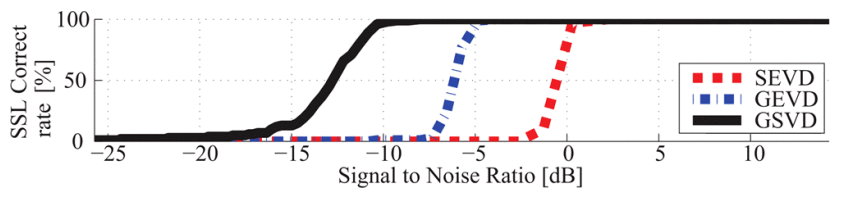
\includegraphics[width=0.75\textwidth]{./nakamura_2012/rate_SNR.png}
\centering
\end{figure}
\cite{nakamura_real-time_2012}

\end{frame}

\section{Simulation}

\subsection{Rectangular Pyramid Array with TDOA}

\begin{frame}
\frametitle{Rectangular Pyramid Array with TDOA}

\begin{columns}

\column{0.7\textwidth}
Based on the paper by Chen \& Xu in 2019.
\begin{itemize}
	\item Calculates the TDOA of all microphone-pairs using GCC-PHAT.
	\item Iteratively solves a model using Newton's method.
	\item Averages four estimates.
\end{itemize}

\column{0.3\textwidth}
\begin{figure}[H]
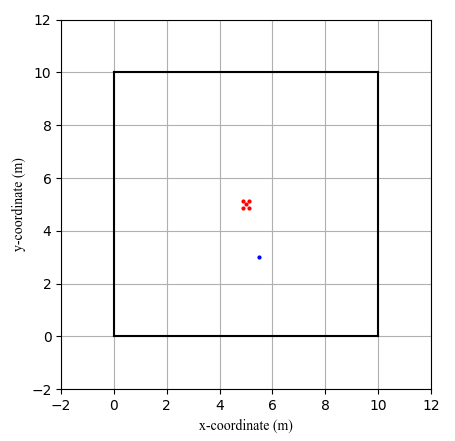
\includegraphics[width=1\textwidth]{../Python/pyramid_robot/room_2d_tight.png}
\centering
\end{figure}

\end{columns}

For each $j$-th microphone:
\begin{equation}
\begin{split}
f_j(x,y,z) &= \sqrt{\left(x-x_j\right)^2 + (y - y_j)^2 + (z - z_j)^2} \\
&- \sqrt{\left(x-x_0\right)^2 + (y - y_0)^2 + (z - z_0)^2}
- c \Delta t_{j0}
\end{split}
\end{equation}

Since it relies on an iterative algorithm, this method tends to fail to converge to a solution, especially for high noise.

\end{frame}

\begin{frame}
\frametitle{Results for Distance}

\begin{figure}[H]
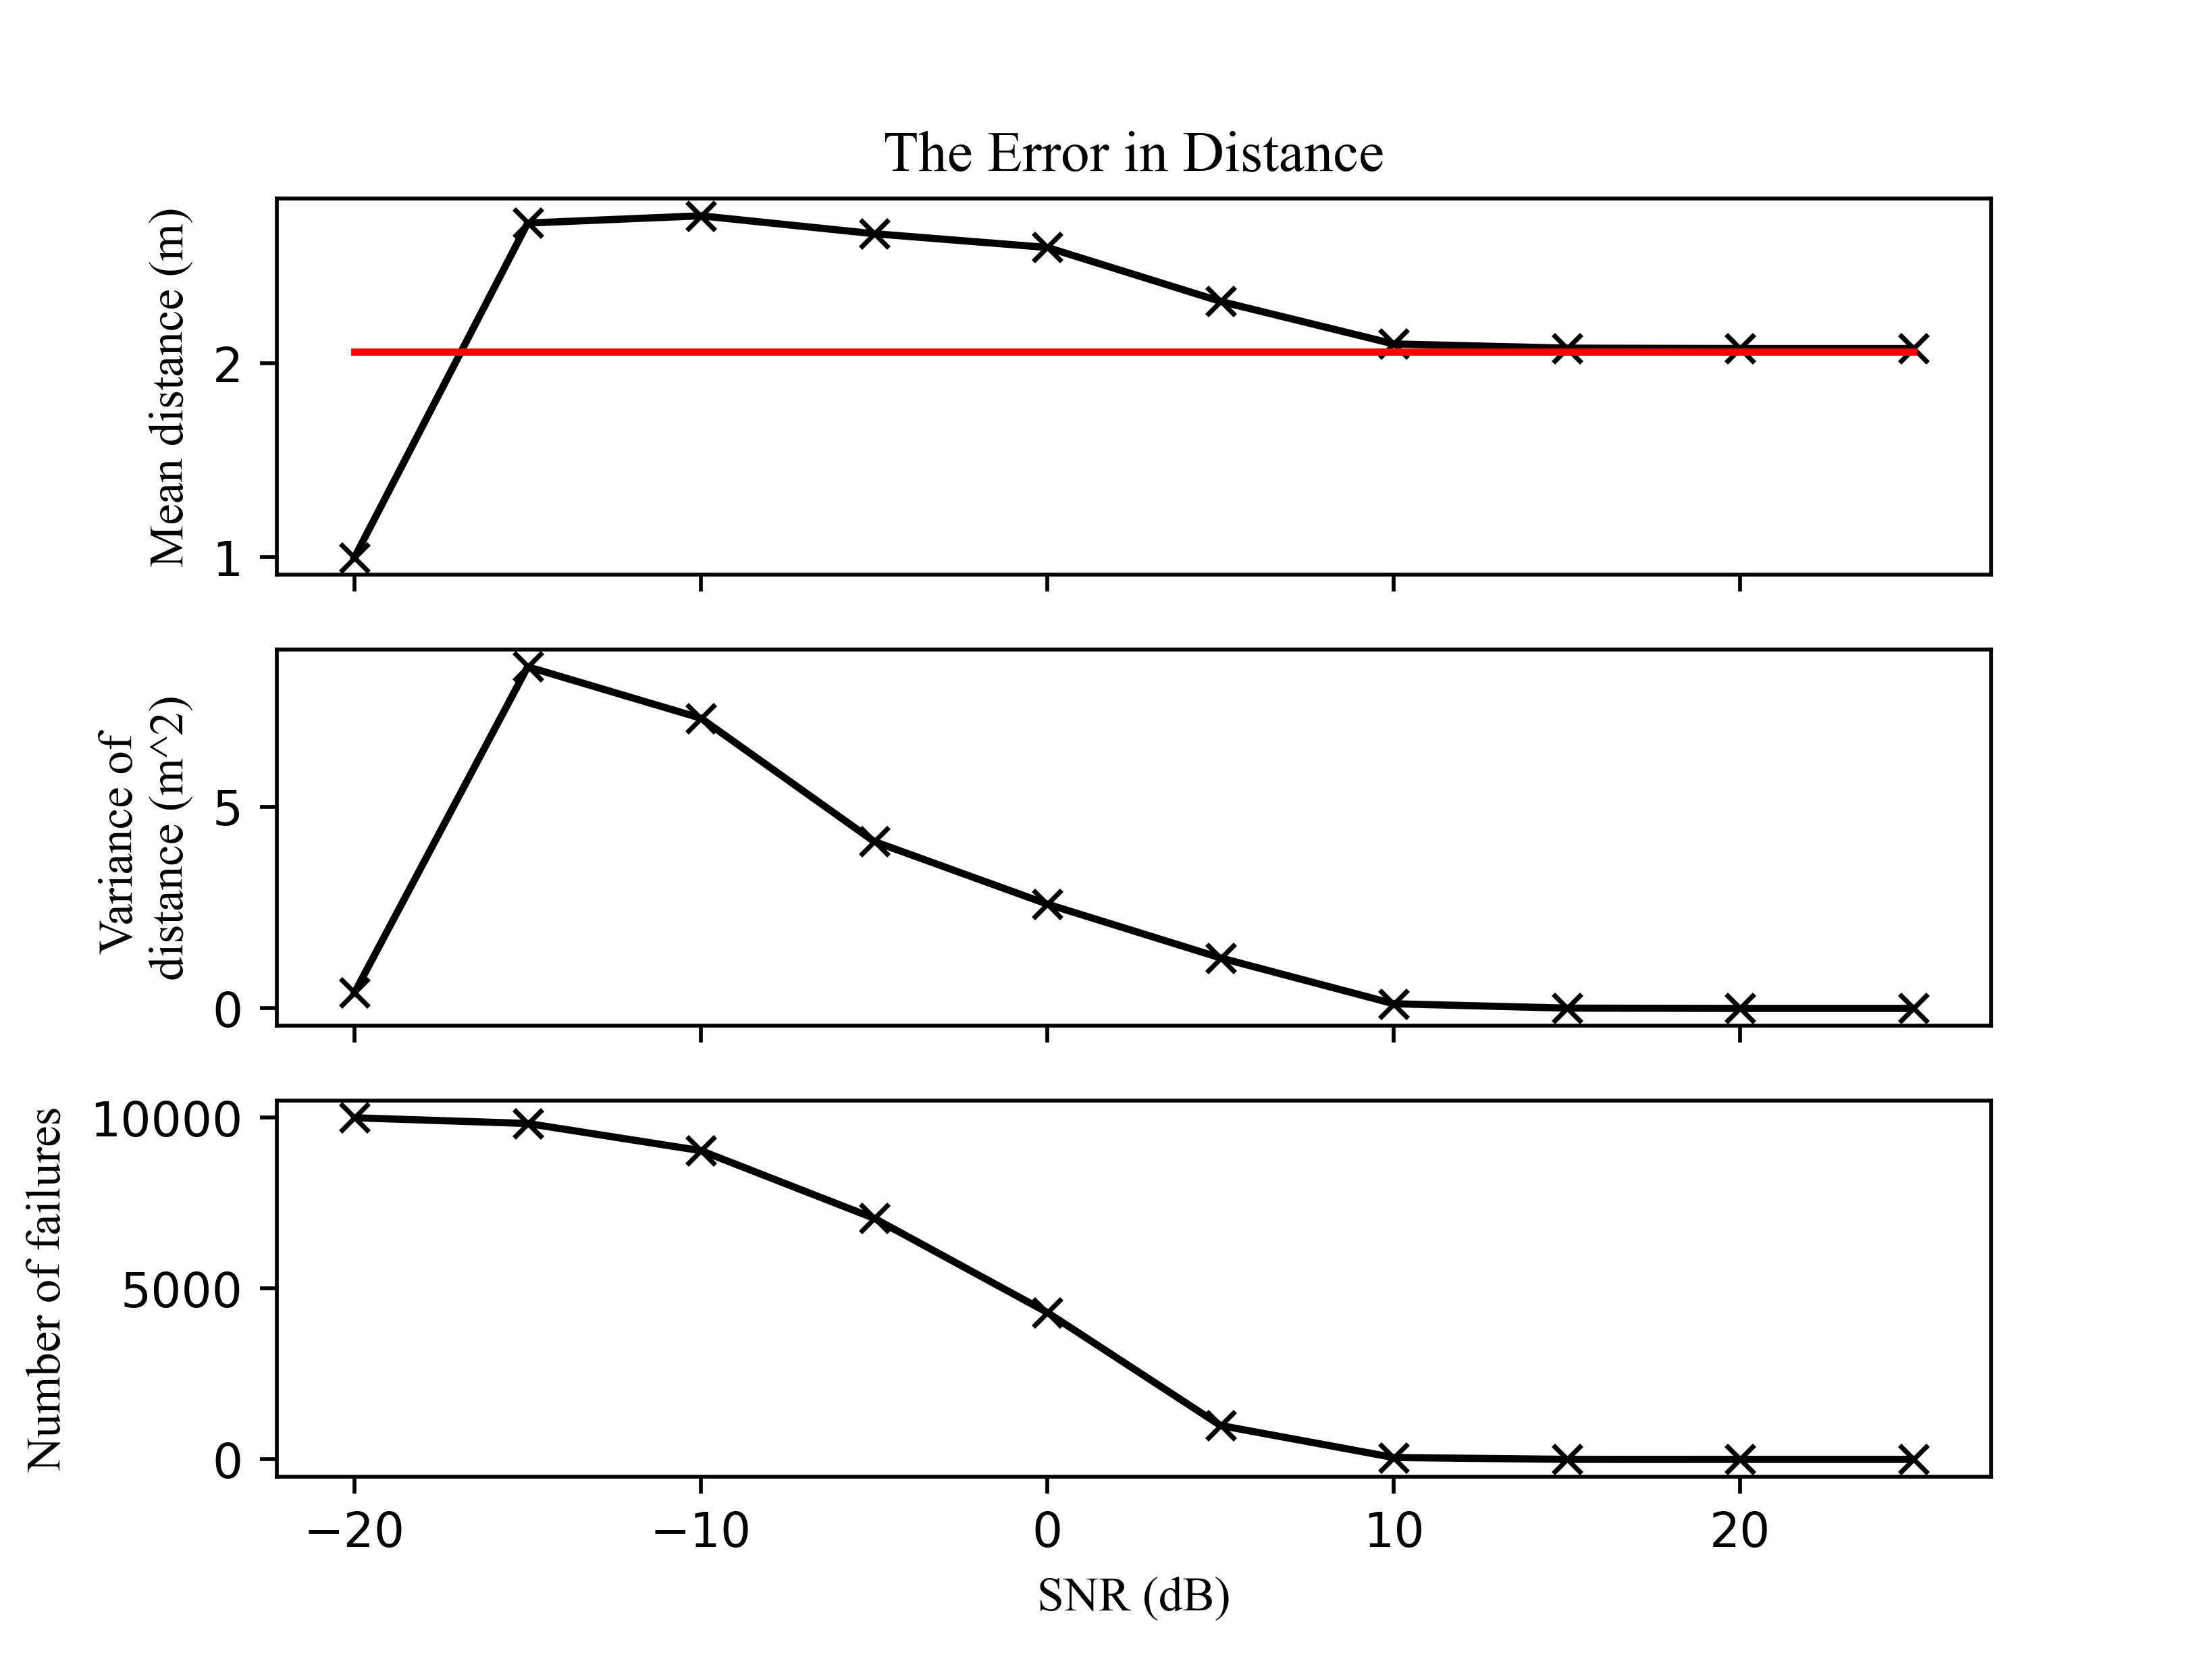
\includegraphics[width=0.9\textwidth]{../Python/pyramid_robot/noise_distance.png}
\centering
\end{figure}

\end{frame}

\begin{frame}
\frametitle{Results for Azimuth}

\begin{figure}[H]
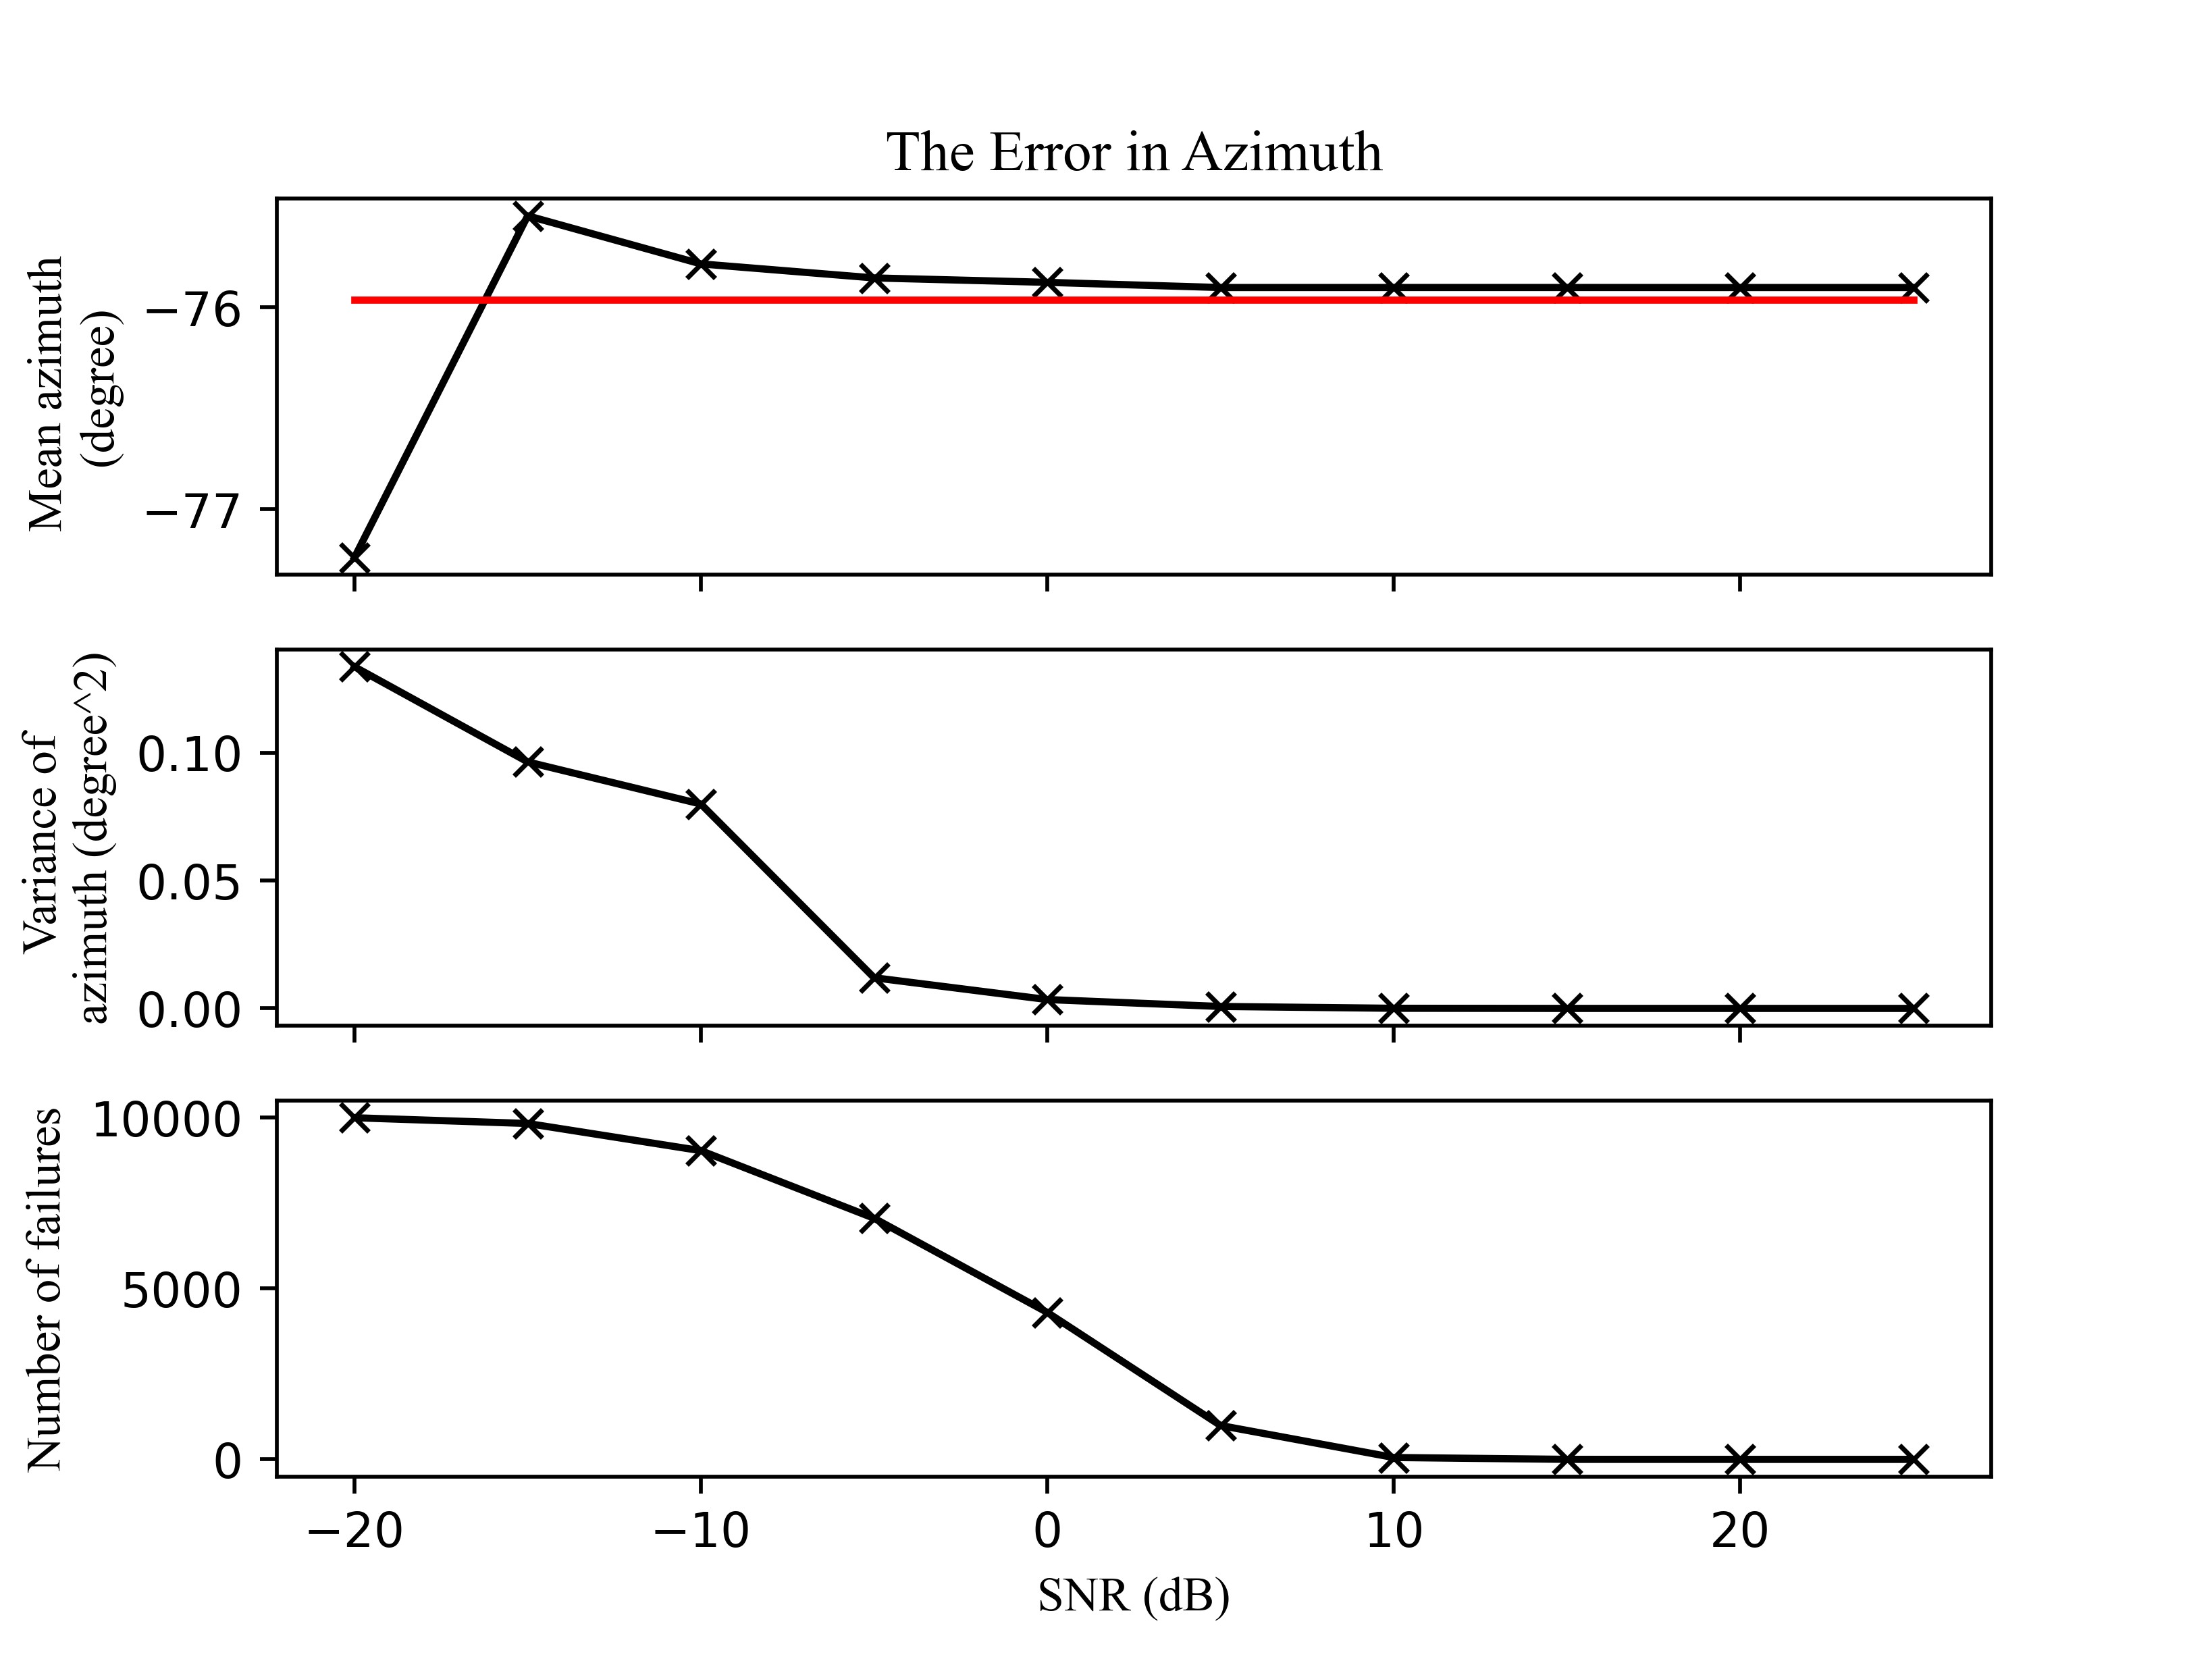
\includegraphics[width=0.9\textwidth]{../Python/pyramid_robot/noise_azimuth.png}
\centering
\end{figure}

\end{frame}

\subsection{Beamforming with SRP-PHAT}

\begin{frame}
\frametitle{Beamforming with SRP-PHAT}

\begin{columns}

\column{0.5\textwidth}
Based on a few papers, mostly the one by Valin et al. in 2007.
\begin{itemize}
	\item The beamformer's energy is computed for every direction in a spherical search-grid of 2562 points.
	\item Estimates the direction as that corresponding to the highest energy in the energy-map.
	\item Only uses a coarse grid.
\end{itemize}

\column{0.5\textwidth}
\begin{figure}[H]
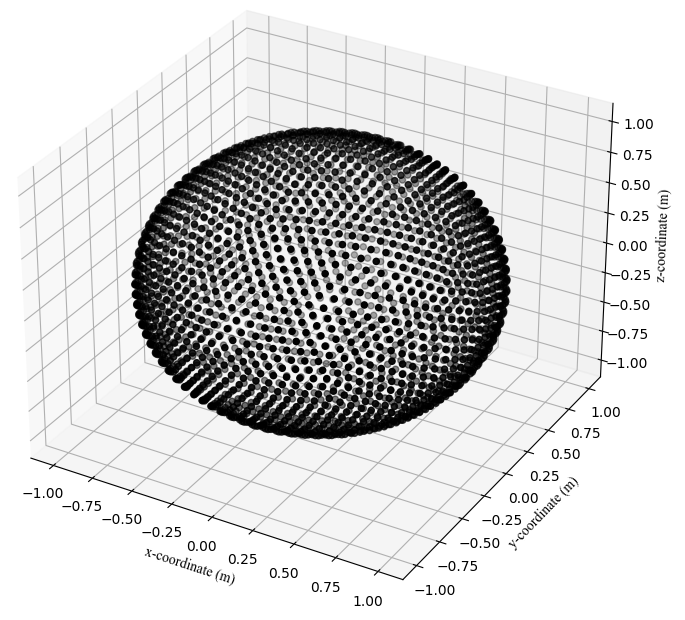
\includegraphics[width=0.9\textwidth]{../Python/srp_phat/grid_tight.png}
\centering
\end{figure}

\end{columns}

\end{frame}

\begin{frame}
\frametitle{Results for Azimuth}

\begin{figure}[H]
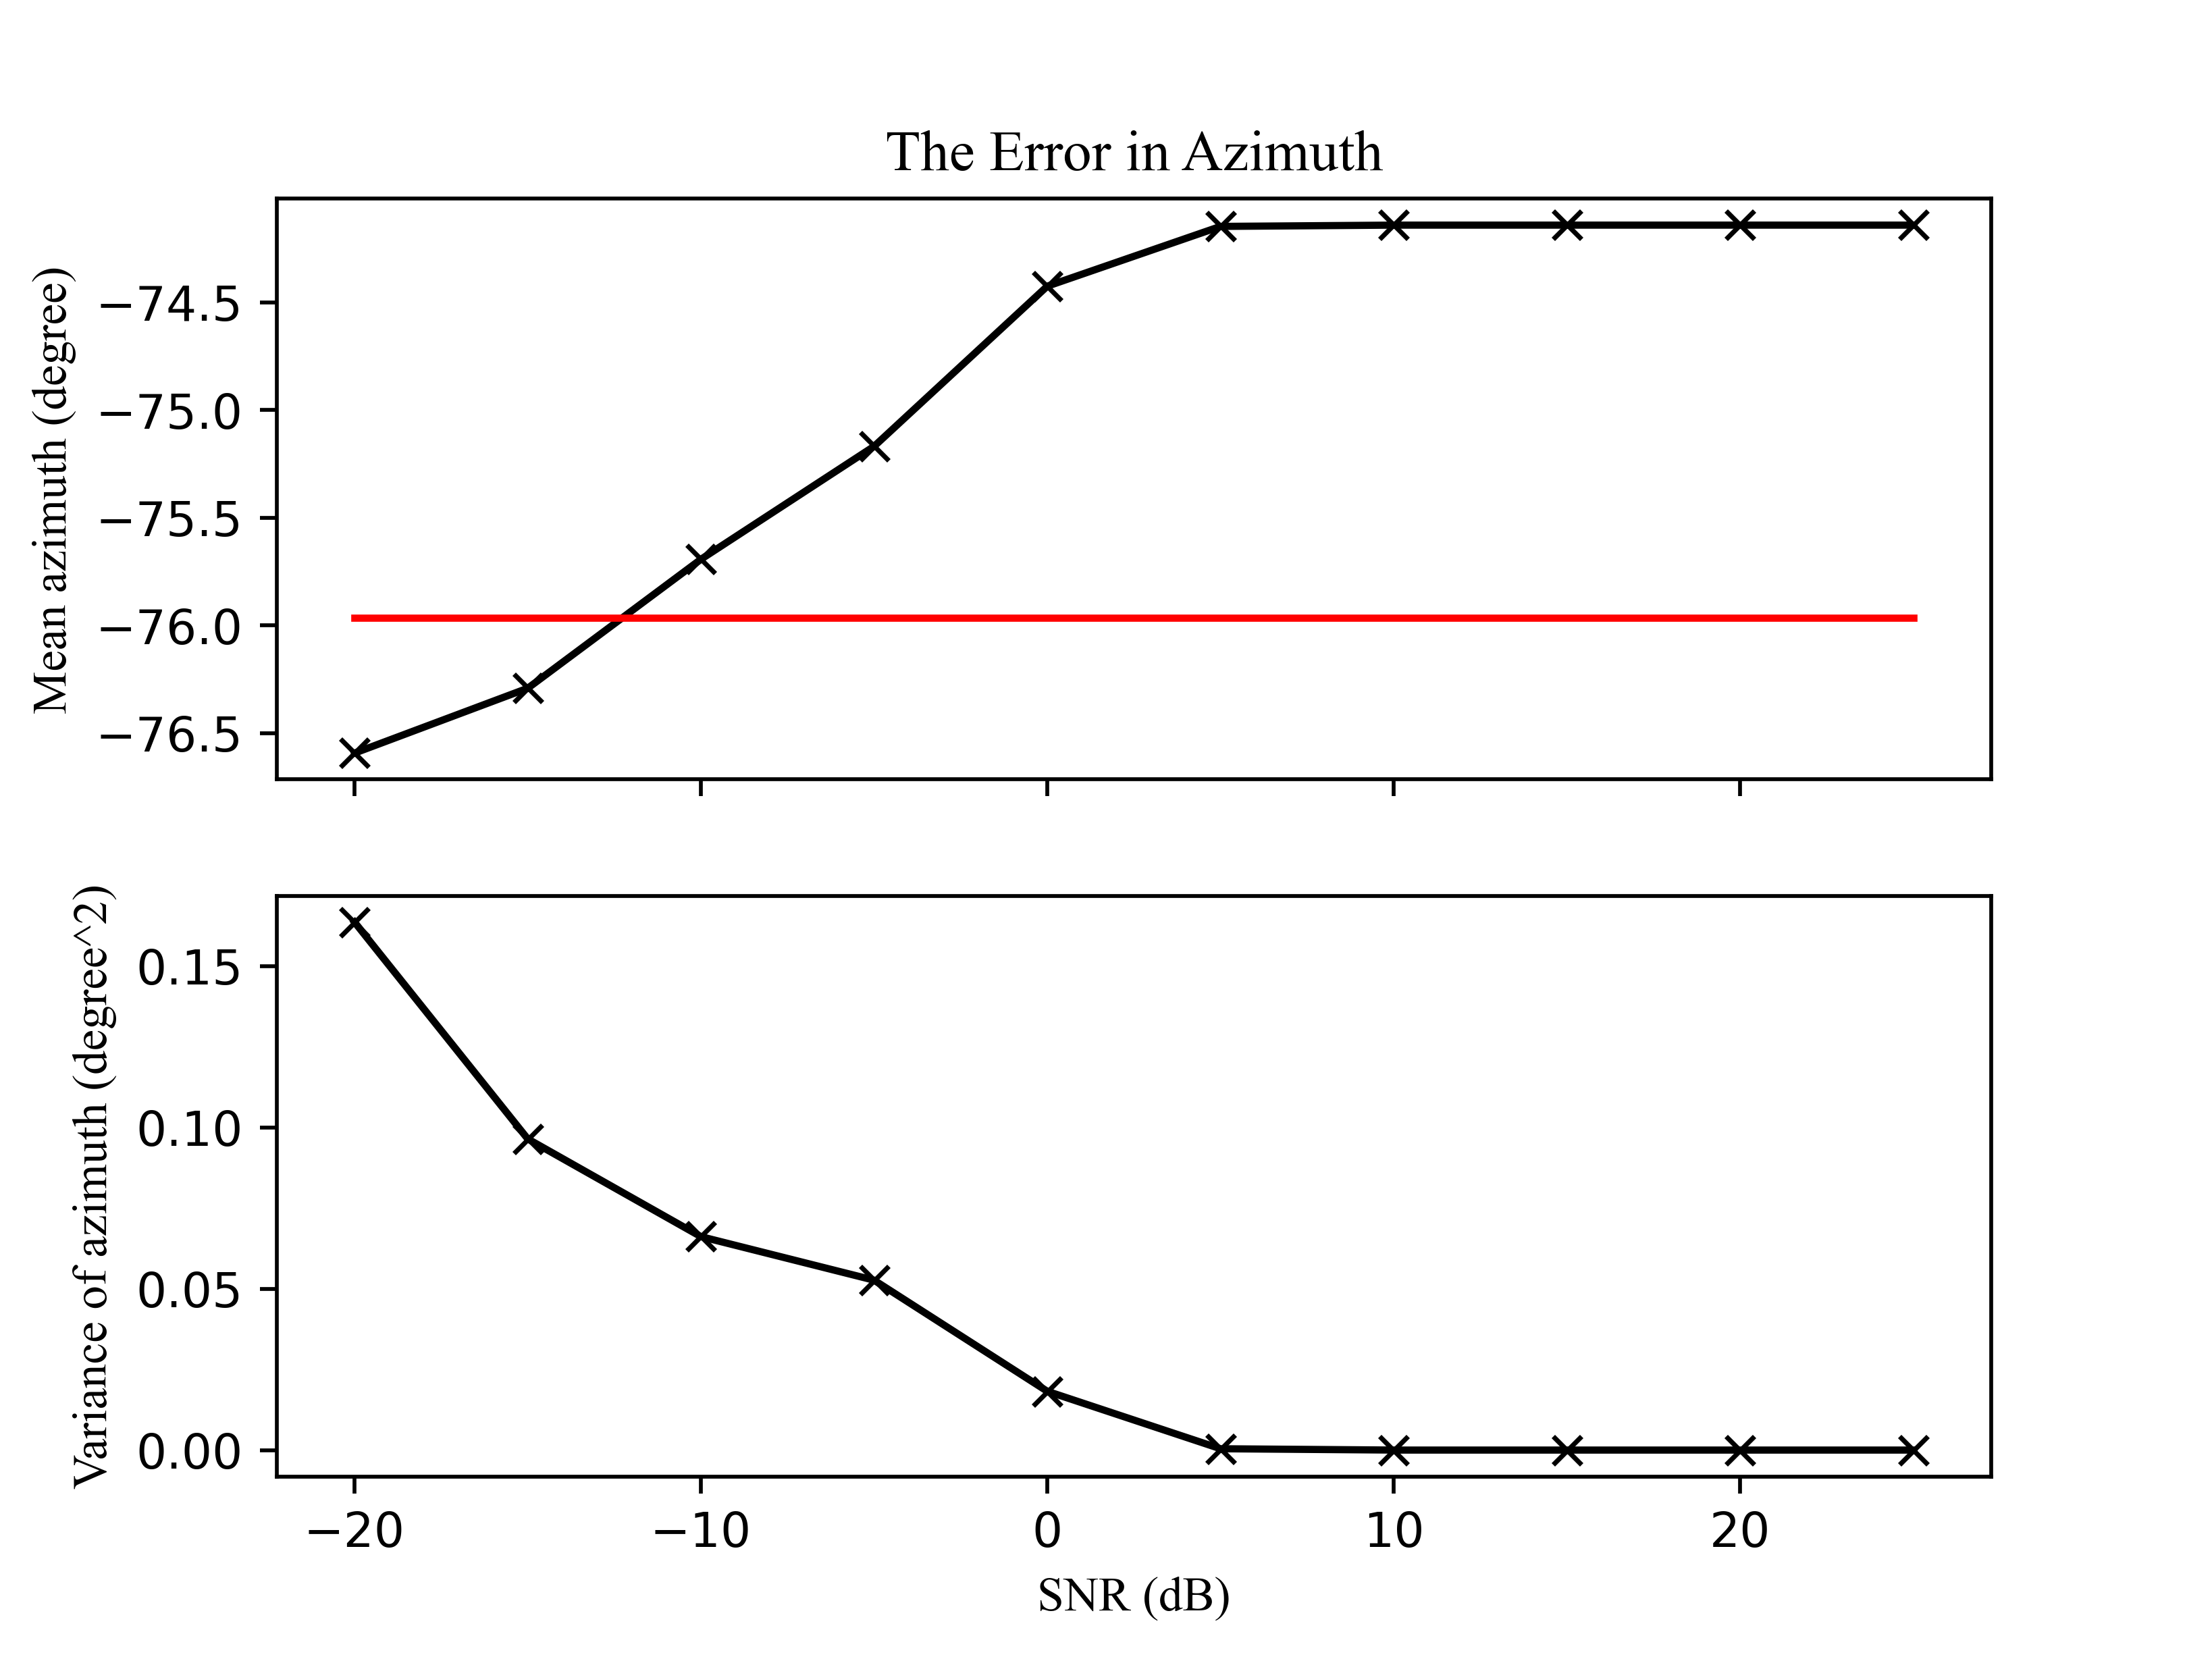
\includegraphics[width=0.9\textwidth]{../Python/srp_phat/noise_azimuth.png}
\centering
\end{figure}

\end{frame}

\begin{frame}
\frametitle{Results for Elevation}

\begin{figure}[H]
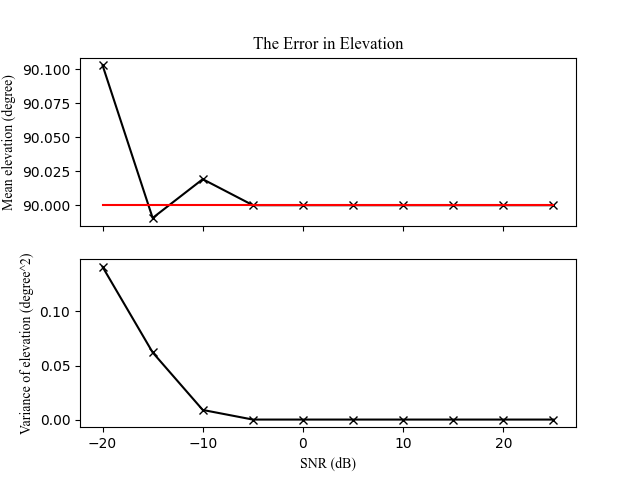
\includegraphics[width=0.9\textwidth]{../Python/srp_phat/noise_elevation.png}
\centering
\end{figure}

\end{frame}

\section{Progress and Schedule}

\begin{frame}
\frametitle{Progress So Far}

\begin{itemize}
	\item Defined the scope.
	\item Completed the literature-review.
	\item Investigated the three main methods.
	\item Did basic simulations of the main literature-examples.
\end{itemize}

\end{frame}

\begin{frame}
\frametitle{Schedule}

\begin{figure}[H]
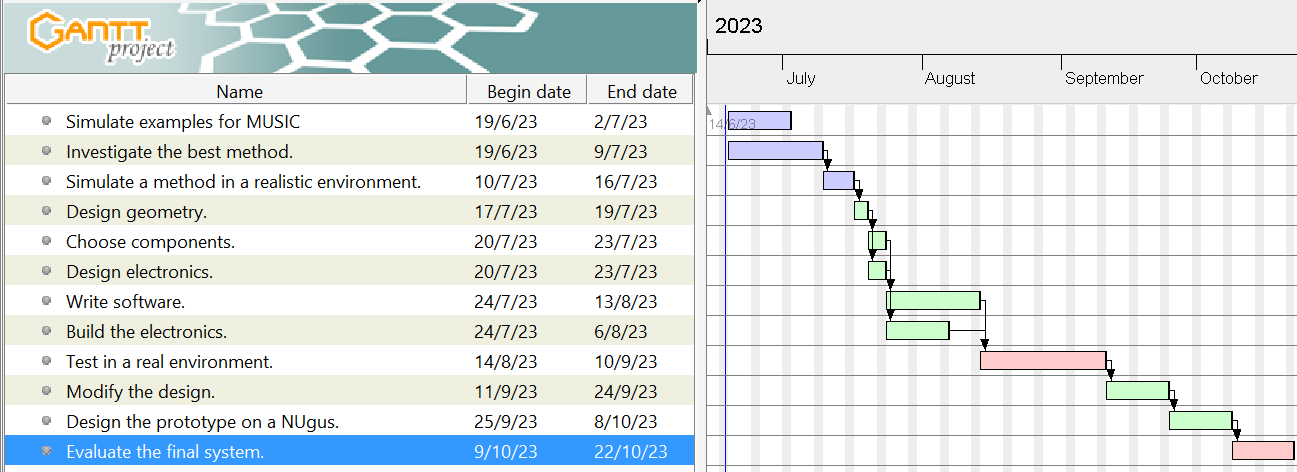
\includegraphics[width=0.9\textwidth]{./gant.png}
\centering
\end{figure}

\end{frame}

\begin{frame}
\frametitle{Schedule}

Winter:
\begin{itemize}
	\item Simulate examples for MUSIC.
	\item Investigate the best method in terms of computation, noise, etc.
	\item Choose a method and simulate it in a realistic environment, e.g. a large hall.
\end{itemize}

\end{frame}

\begin{frame}
\frametitle{Schedule}

Next Semester:
\begin{itemize}
	\item Design the geometry and the set-up of the array.
	\item Choose components, e.g. microcontroller, microphones, etc.
	\item Design the PCB and the physical set-up.
	\item Write software for the microcontroller/processor/etc.
	\item Build the array and the hardware, PCB, etc.
	\item Test the array in a real environment.
	\item Modify the design, software, etc.
	\item Set the design on a NUgus robot.
	\item Test and evaluate the final system in a robotics context.
\end{itemize}

\end{frame}

\begin{frame}
\frametitle{References}
\tiny
\bibliographystyle{plain}
\bibliography{./zotero}

\end{frame}

\end{document}